\documentclass[12pt,a4paper]{article}

% ============================================================
% PACKAGES
% ============================================================

\usepackage[utf8]{inputenc}
\usepackage[T1]{fontenc}
\usepackage{lmodern}

\usepackage[a4paper,margin=1in]{geometry}

\usepackage{setspace}
\onehalfspacing

\usepackage{amsmath,amssymb,amsfonts}
\usepackage{booktabs}
\usepackage{array}
\usepackage{multirow}
\usepackage{graphicx}
\usepackage{float}
\usepackage{enumitem}
\usepackage{xcolor}
\usepackage{hyperref}
\usepackage{url}
\usepackage{xurl}
\usepackage{caption}
\usepackage{fancyhdr}
\usepackage{natbib}

\hypersetup{
    colorlinks=true,
    linkcolor=blue,
    citecolor=blue,
    urlcolor=blue
}

\setlength{\headheight}{14pt}
\pagestyle{fancy}
\fancyhf{}
\rhead{Research Proposal v12}
\lhead{Surrogate Reliability Validation}
\cfoot{\thepage}

% ============================================================
% DOCUMENT
% ============================================================

\graphicspath{{../../results/figures/}{./}}
\begin{document}

\begin{center}
{\LARGE\bfseries Can We Trust the Fast Copy?\\[4pt]}
{\Large\bfseries A Decision-Regret Validation of Machine-Learning Surrogates\\
of Supply-Chain Simulators Under Disruption\par}

\vspace{0.8cm}

\begin{tabular}{ll}
\textbf{Area:} & Supply-chain simulation $\times$ machine learning \\
\textbf{Core method:} & Validation study (DES + surrogate models + conformal prediction) \\ \\
\textbf{Data:} & Synthetic only (one open platform, one disclosed modified fork) \\ \\
\textbf{Compute:} & Laptop-scale (tens of CPU-hours) \\
\end{tabular}

\vspace{0.5cm}
\today
\end{center}

\vspace{0.3cm}

\noindent\fbox{\begin{minipage}{0.95\textwidth}
\textbf{Elevator pitch.} Supply-chain ``digital twins'' increasingly use fast machine-learning (ML) copies of slow simulators to stress-test disruptions. Nobody has ever checked whether those copies stay reliable in exactly the situations they are sold for --- severe, prolonged disruptions far from their training data. We build the missing validation: train standard surrogates on calm-to-mild conditions, test them under disruptions of varying severity \emph{and duration}, and measure not prediction error but \emph{decision regret} --- would a manager following the copy's advice pick the wrong resilience strategy? Outcomes are scored with standard engineering-resilience metrics (resilience-triangle loss, censored time-to-recovery), and ranking-stability claims are protected against both Monte Carlo noise and test multiplicity, with interpretation rules for every outcome pre-specified: the failure branch produces a warning the field needs, the success branch the trust certification it wants.
\end{minipage}}

% ============================================================
\section{Executive Summary}
% ============================================================

Discrete-event simulation (DES) of supply chains is the standard tool for disruption analysis \citep{law2015,kleijnen2015}, but it is too slow for the large-scale what-if testing that resilience management requires. The field's adopted remedy --- and the centerpiece of emerging ``digital twin'' architectures --- is the \emph{surrogate}: an ML model trained on simulator input--output pairs that imitates the simulator in milliseconds. Reviews of digital-twin supply-chain research report that scenario testing for preparedness is a principal advertised capability of these systems \citep{liu2026,tolia2026,meliani2026}.

The reliability of this practice is untested. Surrogates are trained on the simulator's \emph{normal} operating regime, then consulted about \emph{disruptions} --- regimes of congestion, backlog accumulation, and capacity failure that lie outside their training support. In adjacent fields this failure mode is well documented: ML surrogates of physical simulators degrade non-trivially under distribution shift, and conformal-prediction methods have been proposed to detect it \citep{gopakumar2026,zimmel2026}. The supply-chain simulation community, however, has neither imported these tools nor asked the more consequential question: \textbf{does surrogate error change decisions?} A surrogate may be inaccurate yet harmless if its errors never flip the ranking of candidate resilience policies; or it may be deceptively accurate on average yet catastrophic for the decisions that matter. Recent work in predict-then-optimize establishes \emph{decision regret} as the correct evaluation lens for ML embedded in decision pipelines \citep{elmachtoub2022,ban2019,misic2020}, but that literature contains no simulators to validate; the supply-chain simulation literature contains the simulators but no validation.

This proposal fills the intersection. We (i) build a transparent multi-echelon DES with an explicit cost and service layer; (ii) train a standard surrogate battery on calm and mild regimes; (iii) validate the battery under systematically escalating disruption-regime shift using four metrics: prediction error (demoted), \emph{decision regret}, \emph{policy-ranking stability} (with an explicit noise-robustness and multiplicity-control discipline, Section~\ref{sec:metrics}), and \emph{conformal coverage}; and (iv) replicate the validation on a second, independently developed open platform \citep{zhang2026isomorph} to rule out single-simulator artifacts. Interpretation rules for every possible outcome are pre-specified (Section~\ref{sec:results}).

% ============================================================
\section{Motivation and the Adoption--Validation Gap}
% ============================================================

Supply chains are repeatedly disrupted by shocks that propagate through inventory, capacity, and lead-time coupling \citep{hosseini2019,ivanov2021,lee1997}. Simulation-based scenario testing is the standard instrument for preparedness, and digital-twin architectures now position fast ML layers as the mechanism that makes large-scale scenario testing tractable \citep{ivanov2021,ivanov2026}. The adoption is rapid; the validation is not. Table~\ref{tab:gap} lists statements from the 2026 literature in which the field itself concedes the gap.

\begin{table}[H]
\centering
\caption{Printed evidence that surrogate/scenario validation is missing in digital-twin supply-chain research}
\label{tab:gap}
\footnotesize
\begin{tabular}{p{5.2cm}p{9.3cm}}
\toprule
\textbf{Source} & \textbf{Statement} \\
\midrule
Liu et al.\ (2026), SLR of 89 articles \citep{liu2026} & ``\ldots further empirical validation of digital twin applications in supply-chain resilience remains an important avenue for future work.'' \\
\midrule
Huang, Ghadge \& Yates (2026), \emph{IJPR} \citep{huang2026} & ``Behavioural validity and policy/scenario validity were not assessed in this study\ldots'' \\
\midrule
Ivanov (2026), \emph{IJPR} \citep{ivanov2026} & ``Should we be concerned about the validity of AI results?'' \\
\midrule
Soykan \& Rabadi (2026) \citep{soykan2026} & Calls for VVUQ (verification, validation, uncertainty quantification) specific to hybrid AI--digital-twin supply-chain models. \\
\midrule
Meliani \& Sahin (2026) \citep{meliani2026} & Notes absence of convergence in documentation and validation standards for supply-chain digital twins. \\
\midrule
Charoenwut \& Kulvatunyou (2026), \emph{ASME JCISE} \citep{charoenwut2026} & Identifies missing empirical validation in actual supply-chain deployments as a core gap. \\
\bottomrule
\end{tabular}
\end{table}

\textbf{Why regime shift is a distinct threat.} Prior surrogate-uncertainty work in scientific ML addresses smooth covariate drift of PDE/CFD simulators \citep{gopakumar2026,tibshirani2019}. Disruption-regime shift in a DES differs qualitatively: (i) shock onset is abrupt and multi-modal (capacity collapse, demand surge, lead-time inflation), not a gradual covariate rotation; (ii) the system state carries memory --- backlogs and queues accumulate, so errors compound through the policy loop rather than averaging out; (iii) near saturation, simulator responses are discontinuous (a small demand increase can flip a system from clearing to backlog explosion). Whether evaluation methods developed for smooth shift survive this regime is an open question --- and is itself part of the contribution.

% ============================================================
\section{Related Work and Positioning}
% ============================================================

Table~\ref{tab:landscape} maps the four communities whose tooling this proposal connects, and what each leaves undone.

\begin{table}[H]
\centering
\caption{Landscape: what each community has, and what is missing}
\label{tab:landscape}
\footnotesize
\begin{tabular}{p{2.6cm}p{3.4cm}p{4.4cm}p{4.1cm}}
\toprule
\textbf{Community} & \textbf{Vocabulary} & \textbf{Has} & \textbf{Missing} \\
\midrule
Predict-then-optimize / DFL & decision regret, decision-focused learning & Regret as training and evaluation metric \citep{elmachtoub2022,ban2019,misic2020,im2026,fan2026,kaiyrkhan2026,libranke2026,aldridge2026,giannopoulos2026} & No simulators; no disruption regimes; nothing to validate \\
\midrule
Scientific ML & surrogate OOD, conformal UQ & Conformal uncertainty for physics/CFD surrogates; shift protocols \citep{gopakumar2026,zimmel2026,tibshirani2019,vovk2005} & No DES, no queueing/logistics; covariate drift only \\
\midrule
Simulation / OR & metamodel, plausible intervals & Metamodeling foundations \citep{sacks1989,kleijnen2015}; global inference from limited simulation \citep{qiao2026} & Regret there = optimization regret, not decision reliability; no shift-validation studies \\
\midrule
SC / digital twin & digital twin, validation calls & Rapid adoption; explicit calls for validation \citep{liu2026,huang2026,ivanov2026,soykan2026,meliani2026,tolia2026,charoenwut2026} & No surrogate reliability validation; regret only for forecast$\rightarrow$replenishment \citep{li2026ssrn} \\
\bottomrule
\end{tabular}
\end{table}

\subsection{Nearest neighbours and differentiation}

\textbf{Scalese, Narayanan \& Antoniou (2026)} \citep{scalese2026} evaluate a GNN \emph{surrogate of traffic assignment} under distribution shift --- the closest published object. Differences: static network loading vs.\ stochastic discrete-event dynamics with policy feedback; spatial/covariate shift vs.\ disruption \emph{regime change}; and evaluation by predictive accuracy vs.\ by decision regret and policy-ranking stability. Their protocol is a template we extend, not a competitor to the validation itself.

\textbf{P.~Li (2026)} \citep{li2026ssrn} builds a decision-regret benchmark for forecast-driven multi-echelon replenishment on M5/Walmart data. This establishes that regret evaluation has reached supply chains --- for the \emph{forecasting} layer. There is no simulator surrogate, hence no validation of simulation-grounded scenario testing, and no disruption-regime shift. We mirror the benchmark format and cite it as the replenishment-side precedent.

\textbf{Acu\~na (2026)} \citep{acuna2026} integrates conformal probabilistic forecasting with scenario-based planning and sketches regret propagation between layers. This is the forecasting layer again; the simulator-surrogate layer --- where scenario testing actually happens --- is untouched.

\textbf{Mukherjee et al.\ (2026)} \citep{mukherjee2026} test inventory policies across demand families (a useful shift-protocol design). No surrogate of a simulator is involved. \textbf{Shen (2026)} \citep{shen2026} bounds decision regret by surrogate calibration gap --- theoretical support we import for H4 below. \textbf{Qiao, Eckman \& Nelson (2026)} \citep{qiao2026} provide guaranteed global inference from limited simulation within the OR community --- inference about the simulator, not reliability of an ML copy under regime change.

\subsection{Novelty claim (scoped)}

To our knowledge, no study systematically validates whether ML surrogates of supply-chain simulators remain \emph{decision-reliable} under disruption-regime shift, and no evaluation protocol combining decision regret, noise-aware and multiplicity-controlled ranking-stability, and conformal coverage exists for this setting. All constituent methods are imported and cited; the contribution is the validation object, the regime-shift protocols, and the verdict --- not the invention of metrics. A four-direction search of the literature (ML; scientific ML; simulation/OR; SC/digital twin), documented in a search log with search strings and dates, underlies this claim; a final forward-citation re-check is scheduled before submission.

% ============================================================
\section{Research Questions}
% ============================================================

\begin{description}[leftmargin=1.2cm]
\item[RQ1.] When surrogates trained on calm/mild regimes are queried on escalating disruption scenarios, how large are their errors on fill rate, backlog, and cost --- and how does error scale with severity? (Baseline; expected and not sufficient.)
\item[RQ2.] \textbf{Do surrogate errors change decisions?} Does the policy selected using the surrogate differ from the policy selected using the true simulator, and at what severity does the \emph{ranking of resilience policies} begin to flip --- among policy pairs that the simulator can distinguish at the stated replication budget, under false-discovery-rate control (Section~\ref{sec:metrics})?
\item[RQ3.] \textbf{Can conformal prediction detect unreliability?} Do conformal intervals, calibrated on calm data, maintain their coverage guarantee under disruption shift --- i.e., can a twin \emph{know when it does not know}?
\end{description}

\textbf{Hypotheses.} H1: prediction error grows monotonically with severity, with model-class-specific failure signatures (Section~\ref{sec:battery}). H2: rank flips among \emph{decidable} policy pairs (practical margin $\delta$, BH-controlled at $q=0.10$) concentrate at high severity and are more frequent for surrogates over backlog-type outputs than flow-type outputs, attributed by a leave-one-output-true ablation (each output's surrogate prediction is swapped for ground truth in turn, and the resulting change in flip rate attributed to that output). H3: conformal coverage deficit grows with severity; a covariate-shift-weighted variant \citep{tibshirani2019} partially repairs it. H4 (the interesting one): decision regret is \emph{not} a monotone function of prediction error --- some accurate-on-average surrogates cause large regret on specific regimes --- establishing that decision-level evaluation is necessary, not decorative \citep{shen2026}. H5 (pre-registered): decision regret is non-monotone in $(\sigma, D)$ jointly, peaking at intermediate combinations rather than at either extreme, for (at least) one of two candidate mechanisms this design does not pre-commit between: (a) \emph{lead-time mismatch} --- regret peaks when $D$ is comparable to a node's replenishment lead time (Table~\ref{tab:duration}), where ordering-policy timing matters most and dynamics are most nonlinear; or (b) a \emph{recoverability edge} --- near $(\sigma,D)$ combinations where disruption-induced backlog approaches what post-restoration capacity can drain within the observation window, policy differentiation compresses and regret falls, a two-dimensional analogue of the collapse-driven convergence identified in the stability-boundary note (Section~\ref{sec:compute}). Confirming either shape decouples regret from error twice over, sharpening H4 into a specific, falsifiable prediction rather than a general caution; the leave-one-output-true ablation (H2) is planned to help distinguish the two mechanisms if H5 is confirmed.

% ============================================================
\section{Method}
% ============================================================

\subsection{Architecture: two simulators}\label{sec:architecture}

A single-simulator validation is vulnerable to the objection that findings are artifacts of one model. The design therefore uses two:

\begin{itemize}
\item \textbf{Simulator A (primary, ground truth).} Our own SimPy DES \footnote{\url{https://simpy.readthedocs.io}} --- small (one supplier tier $\rightarrow$ two regional DCs $\rightarrow$ retail tier), $(s,S)$ replenishment \citep{law2015}, stochastic demand and lead times, and an explicit cost layer (holding, backlog penalty, transport). Disruptions are timed, bounded-duration events --- a severity $\sigma$ applied for a duration $D$ then restored, rather than a permanent regime change --- per the design rationale in Section~\ref{sec:compute}. Baseline capacity margin is set generously (2--3$\times$ nominal demand), a lesson pulled directly from Simulator B's stability-boundary characterization (Section~\ref{sec:compute}), so the severity dial spans meaningful degradation across the full range instead of saturating early. Full transparency permits verification against analytical extreme-condition tests \citep{law2015,kleijnen2015}.
\item \textbf{Simulator B (replication).} ISOMORPH \citep{zhang2026isomorph} --- an independent, open-source (MIT) supply-chain simulator on a real freight-city network, with $(s,S)$ policies (global and per-tier), Dijkstra routing, parametric demand-shock/capacity knobs, and released scenario sweeps. ISOMORPH does not track monetary costs; the replication therefore measures \emph{service-level regret} (Section~\ref{sec:metrics}), which is the standard resilience objective in disruption studies and is fully supported by its outputs (fill rates, backorders, lead times). The released sweeps and datasets are built for ISOMORPH's own time-series-forecasting benchmark (single seed, full-horizon rollouts) and are used here only to calibrate severity-to-knob mappings and for sanity-checking, not as reusable regret-pipeline data; every policy-comparison run the validation needs is generated fresh at the run length fixed empirically for this purpose (Section~\ref{sec:compute}). Timed disruptions on B use a third disclosed patch (Section~\ref{sec:compute}) rather than the platform's own targeted-edge-cut extension, which was considered and rejected for this role: it is currently non-functional (the extension's script imports a module absent from the public release) and, independently of that, binary rather than graded (edges are excluded outright, not partially throttled), which would give at most a handful of achievable severity levels regardless.
\end{itemize}

The validation's headline results must replicate across both. Cost-based regret (A) and service-based regret (B) are reported as complementary views.

\subsection{Decision layer}

The policy set $\Pi$ is a grid of $(s,S)$ parameters (crossed, in Simulator A, with a binary dual/option-sourcing choice). For each scenario $x = (\sigma, D, \text{type})$ --- a severity level, a disruption duration, and a shock type (Section~\ref{sec:shift}):

\begin{equation}
\pi^{\star}(x) \in \arg\min_{\pi \in \Pi} \; TC_{S}(x,\pi) \quad \text{s.t.} \quad SL_{S}(x,\pi) \geq SL_{\min},
\end{equation}
\begin{equation}
\hat{\pi}(x) \in \arg\min_{\pi \in \Pi} \; \widehat{TC}(x,\pi) \quad \text{s.t.} \quad \widehat{SL}(x,\pi) \geq SL_{\min},
\end{equation}
where $S(\cdot)$ denotes the true simulator and $\widehat{\cdot}$ the surrogate. $\hat{\pi}(x)$ is the manager following the fast copy's advice; $\pi^{\star}(x)$ is the advice the slow truth would have given.

\subsection{Surrogate battery}\label{sec:battery}

\begin{table}[H]
\centering
\caption{Surrogate battery and expected failure signatures}
\label{tab:battery}
\footnotesize
\begin{tabular}{p{3.2cm}p{5.0cm}p{6.0cm}}
\toprule
\textbf{Model} & \textbf{Role} & \textbf{Anticipated failure mode under regime shift} \\
\midrule
Linear regression & Misspecified baseline & Smooth extrapolation of a saturating system \\
Random forest \citep{breiman2001} & Nonlinear workhorse & Piecewise-constant artefacts; no extrapolation beyond leaf ranges \\
XGBoost / LightGBM \citep{chen2016} & Current default in practice & Confidence far outside training support; discontinuity smoothing \\
Gaussian process \citep{rasmussen2006,sacks1989} & Benchmarks uncertainty & Overconfident posterior in extrapolation unless kernel is regime-aware \\
Small MLP (2$\times$64) & Smooth interpolator & Plausible-looking but wrong dynamics near saturation \\
\bottomrule
\end{tabular}
\end{table}

Inputs: scenario parameters (severity $\sigma$, duration $D$, shock type, demand parameters, $(s,S)$, capacity), plus policy. Outputs: window-limited primary metrics and censored time-to-recovery (Section~\ref{sec:metrics}), total cost (A only). Hyperparameters via nested cross-validation on the \emph{training} regime only --- no peeking at shifted data.

\subsection{Shift protocols}\label{sec:shift}

\begin{table}[H]
\centering
\caption{Distribution-shift protocols (train support $\rightarrow$ test support)}
\label{tab:shift}
\footnotesize
\begin{tabular}{p{3.0cm}p{5.4cm}p{5.8cm}}
\toprule
\textbf{Protocol} & \textbf{Training} & \textbf{Testing} \\
\midrule
P1: Severity/duration extrapolation & Calm + mild only ($\sigma \leq 0.2$, $D \in \{\text{short, medium}\}$; Table~\ref{tab:regimes}) & Full grid $\sigma \in (0.2, 1]$ $\times$ all $D$, binned; sensitivity variant trained on $\sigma \leq 0.3$ \\
P2: Type transfer & Demand-surge shocks only & Capacity-failure and lead-time-inflation regimes (and vice versa) \\
P3: Structure transfer (A) & Fixed topology & Modified topology (link capacity halved; a DC removed) \\
P4: Compound shift (A) & Single-shock regimes at short/medium $D$ & Simultaneous demand + capacity shocks, jointly varying $(\sigma, D)$ \\
\bottomrule
\end{tabular}
\end{table}

Severity $\sigma \in [0,1]$ and duration $D \in \{\text{short, medium, long}\}$ ($\sim$14/30/90 days; Table~\ref{tab:regimes}) jointly map to concrete, timed knobs (e.g., $\sigma=0.8$, $D=\text{long}$ = an 80\%-of-margin capacity cut sustained for 90 days, then restored), so that ``severe'' and ``prolonged'' are each a reproducible quantity, not an adjective. Disruptions are bounded events applied within a fixed run length $L$ (Section~\ref{sec:compute}) and then restored, not permanent regime changes --- the design rationale for this choice, and what happens on this network when regimes are instead permanent, is given in Section~\ref{sec:compute}. Training data are generated by Latin Hypercube Sampling over the training support (severity continuous, duration restricted to short/medium so the surrogate sees genuine disruption dynamics without the long, policy-stressing durations reserved for testing) with replicated seeds; test grids are factorial and binned over severity $\times$ duration $\times$ shock type $\times$ policy grid, since the flip tables (Section~\ref{sec:metrics}) need discrete, interpretable cells rather than a continuous LHS scatter. All simulator estimates are replicated across 30 seeds and reported as mean $\pm$ 95\% CI; stochasticity is verified by checking seed-to-seed variance before any surrogate is trained. Because the training-support choice (P1) is itself an experimental degree of freedom, a sensitivity variant with the wider support ($\sigma \leq 0.3$) is run and reported; conclusions that flip between the two variants are flagged rather than hidden.

\subsection{Evaluation metrics}\label{sec:metrics}

\textbf{Window-limited outcome metrics.} Every policy-comparison run uses one fixed length $L$ (warm-up + longest disruption duration + a post-restoration recovery-observation window; Section~\ref{sec:compute}), identically defined whether the run is generating training data or test data --- the single evaluation-window definition an earlier version of this design left unstated, and would otherwise have confounded with regime shift itself. Primary outcomes are computed over the post-warm-up portion of this fixed window and are therefore always well-defined regardless of whether the system has fully recovered by the end of it: cumulative unmet demand, and the \emph{resilience-triangle} area \citep{bruneau2003,henry2012} --- the integral of lost functionality ($1-$fill rate) over the window, a standard engineering-resilience metric that is monotone in severity and duration by construction. Peak backlog within the window is reported alongside. \emph{Time-to-recovery} (first day fill rate returns to within a practical margin of its pre-disruption level) is reported as a secondary metric and is right-censored when recovery does not occur within $L$ --- standard reliability-engineering practice \citep{henry2012} for exactly the situation severe, prolonged $(\sigma,D)$ combinations produce.

\textbf{Prediction error} (reported, demoted): $MAE$, $RMSE$ per output per severity bin.

\textbf{Decision regret} --- the primary metric. All simulator evaluations are run under \emph{common random numbers} \citep{law2015}: the same seed set is used to estimate performance under $\hat{\pi}(x)$ and $\pi^{\star}(x)$, so regret is computed from paired per-seed differences,
\begin{equation}
DR(x) = \frac{1}{R}\sum_{r=1}^{R}\Big[ TC\big(x,\hat{\pi}(x);\epsilon_r\big) - TC\big(x,\pi^{\star}(x);\epsilon_r\big) \Big] \;\geq\; 0,
\end{equation}
with the paired 95\% CI over seeds. For the cost-free Simulator B, the service-level analogue is
\begin{equation}
DR^{SL}(x) = \frac{1}{R}\sum_{r=1}^{R}\Big[ SL\big(x,\pi^{\star}(x);\epsilon_r\big) - SL\big(x,\hat{\pi}(x);\epsilon_r\big) \Big] \;\geq\; 0.
\end{equation}
Regret is zero when the copy's advice coincides with the truth's; it is the operational price of trusting the copy. Pairing removes seed-level noise from the comparison; the remaining uncertainty is reported and propagated into all flip counts below.

\textbf{Noise-aware ranking stability.} Comparing rankings estimated from finite Monte Carlo runs invites two confounds: near-tied policies produce apparent flips from simulation noise alone, and with hundreds of simultaneous pairwise tests, some pairs appear distinguishable by chance alone. Four safeguards make the flip statistic interpretable:

\begin{enumerate}
\item \emph{Decidable pairs with a practical margin.} A pair $(\pi_a,\pi_b)$ is \textbf{decidable} in a severity $\times$ shock-type cell if the lower bound of the paired 95\% CI (common random numbers \citep{law2015}) of the per-seed performance difference exceeds a pre-registered practical margin $\delta$ --- the smallest cost/service difference that would matter to a decision-maker (default: 1\% of baseline total cost, or 0.5 percentage points of fill rate; sensitivity over $\delta$ reported). The margin converts ``statistically distinguishable'' into ``decision-relevant and distinguishable.''
\item \emph{Multiplicity control within families.} All $\binom{|\Pi|}{2} = 300$ pairwise tests within a cell (severity $\times$ shock type) form one family; families are corrected separately because the headline claims are per-cell flip rates. False discovery rate is controlled by Benjamini--Hochberg at $q=0.10$ \citep{benjamini1995,benjamini2001}. FDR (rather than family-wise) control is chosen deliberately: the flip statistic is an aggregate rate, so FDR bounds precisely the quantity that matters --- the expected fraction of decidable pairs that are noise; BH is valid under the positive dependence that common random numbers induce among tests sharing policies \citep{benjamini2001}; and family-wise control would shrink the decidable set at high-severity bins, biasing the validation by scope reduction rather than evidence. Holm correction \citep{holm1979} is reported as a family-wise sensitivity for headline tables; Benjamini--Yekutieli if dependence diagnostics warrant. Undecidable pairs are excluded from flip counting and reported as the \emph{undecidable mass} per cell, which bounds how finely the simulator can discriminate policies at all.
\item \emph{Placebo noise floor.} Before trusting any surrogate flip rate, the surrogate is replaced by an \emph{independent second Monte Carlo sample of the true simulator} at the same evaluation budget and run through the identical decidability-plus-flip pipeline. The resulting rate is the pure noise floor --- residual noise flips among falsely decidable pairs. Headline results are reported as \emph{excess flips over placebo}, with the placebo rate printed beside every flip table. BH bounds the contamination analytically; the placebo measures it empirically.
\item \emph{Adaptive deepening} (budget permitting): for near-tie top-1 contenders, replication is increased until the pair is decidable at the BH-adjusted threshold or a preset replication cap is hit; the BH correction is recomputed once on the final replication counts to avoid forking-path ambiguity.
\end{enumerate}

At each severity bin $\sigma$, we report Kendall's $\tau$ between the simulator's and the surrogate's rankings over decidable pairs, plus a binary \emph{top-1 flip indicator} (meaningful only when the top-2 pair is decidable). This yields the paper's centerpiece: a severity $\times$ model table of noise-corrected, multiplicity-controlled policy-ranking flips. Every flip table is accompanied by a per-cell transparency table (number of tests, BH threshold, decidable count, undecidable mass, placebo rate).

\textbf{Conformal coverage under shift.} Split-conformal intervals \citep{vovk2005,angelopoulos2023}: calibration residuals $r_j = |y_j - \hat f(x_j)|$ on held-out calm data; quantile $\hat q_{\alpha}$ at level $1-\alpha$; interval $\hat f(x) \pm \hat q_{\alpha}$. We report the \emph{coverage deficit}
\begin{equation}
\Delta(\sigma) = (1-\alpha) - \widehat{\mathrm{cov}}(\sigma),
\end{equation}
where $\widehat{\mathrm{cov}}(\sigma)$ is empirical coverage at severity $\sigma$. Perfect $\Delta \equiv 0$ means the twin's error bars remain honest; growing $\Delta$ means disruption silently breaks the guarantee. A covariate-shift-weighted variant \citep{tibshirani2019} is applied as a repair attempt, reported before/after. Because test points at a given severity share simulation noise, conformal coverage is computed across independent seeds, and the seed count per bin is chosen so that binomial coverage estimates are stable.

\subsection{Validation protocol}\label{sec:audit}

\begin{enumerate}
\item Implement Simulator A; verify via extreme-condition and trace checks \citep{law2015}; sanity-match bullwhip/backlog behaviour against literature ranges \citep{lee1997}; run a warm-up pilot mirroring Simulator B's methodology (5 seeds, calm and one severe timed disruption, ensemble-mean trajectory) to fix A's own warm-up margin and run length $L$.
\item Generate training data: LHS over the training support ($\sigma \leq 0.2$, $D \in \{\text{short, medium}\}$), $\approx$8{,}000--10{,}000 runs (A), replicated seeds; for B, released sweeps are used only to calibrate severity-to-knob mappings and for sanity-checking (Section~\ref{sec:compute}) --- the $\approx$2{,}000--3{,}000 training runs are freshly generated at the fixed run length $L$ established there.
\item Fit the battery (Table~\ref{tab:battery}) with nested CV on training regimes.
\item Generate test grids under P1--P4; evaluate error, $DR$, $\tau_\sigma$, decidable-pair flips (practical margin $\delta$, BH-controlled, with placebo floor), and $\Delta(\sigma)$ per bin; recompute the BH correction once on final replication counts after adaptive deepening.
\item Apply conformal calibration (naive and shift-weighted); report coverage before/after repair.
\item Replicate headline results on Simulator B.
\item Assemble the verdict table and release package (code, seeds, configurations, run data) under open license.
\end{enumerate}

\subsection{Compute budget}\label{sec:compute}

Simulator A: $\sim$10$^4$ runs at 0.2--1\,s each $\Rightarrow$ single-digit CPU-hours; placebo and adaptive-deepening replications are budgeted at a further 2$\times$ margin.

Simulator B: benchmarked empirically rather than assumed.\footnote{Run directly by the author on Google Colab (CPU runtime); command and console output are logged in the project's reproducibility materials.} All benchmarking and pilot runs use \texttt{pipeline\_mult=7} throughout: ISOMORPH's own built-in default is 0 (a reactive shipping rule), while 7 selects the proactive rule its released baseline and scenario-sweep datasets actually use, so every figure in this section stays comparable to the released baseline rather than resting on an unstated choice. A full 7{,}300-day rollout on the released baseline configuration (C=50 catalogue, seed 2025) --- ISOMORPH's own default horizon, sized for its time-series-forecasting benchmark --- completed in 409.9\,s (17.8 simulated days/s), with unperturbed fill rate 0.918 (range 0.873--0.952 across items); this per-day rate is what the rest of this budget scales from.

\paragraph{A horizon-independent shock generator (patch 1).} The released global-shock generator places a horizon-independent count of long events (5--11 events, each 180--1{,}100 days) uniformly across whichever run length is requested; at short horizons this compounds into unrepresentative, near-permanent disruption rather than the sparse pattern the 7{,}300-day design intends. A single-line, disclosed patch --- scaling event duration by (requested days)/7{,}300 --- is applied in a public fork; the patch is a mathematical no-op at the original 7{,}300-day horizon (scale factor 1.0), so it reproduces the released baseline and scenario-sweep datasets exactly and only changes behavior at other horizons.

\paragraph{One fixed run length, not a training/test split.} A pilot warm-up study (5 seeds, ensemble-averaged fill rate, shock-free vs.\ a permanent capacity cut; Figure~\ref{fig:warmup}) found the calm regime stabilizes by $\sim$day 100. Combined with the duration ladder fixed in Table~\ref{tab:regimes} ($D \in \{14, 30, 90\}$ days) and a further $\sim$100-day post-restoration window so time-to-recovery has a fair chance to resolve before censoring (Section~\ref{sec:metrics}), every policy-comparison run on B uses one fixed length $L = 400$ days (warm-up $+$ longest duration $+$ recovery window; $L=300$ in v10--v11, raised after Gate~4, below), applied identically whether the run generates training or test data --- this is what eliminates the horizon-definition confound an earlier version of this design would otherwise have introduced by using different run lengths (200 vs.\ 700 days) for the two. At $L=400$, per-run cost is $\approx$22.5\,s (400/7{,}300 of 409.9\,s), so the $\approx$2{,}000--3{,}000 training runs cost $\approx$12--19 CPU-hours; at 2 parallel workers (the Colab default) this is $\approx$6--9 wall-clock hours, split across checkpointed sessions. $L=400$ is confirmed by the Gate~4 severity scan below: at $L=300$ every 90-day cell at overload $\nu\geq0.5$ is right-censored, at $L=400$ only the most extreme 90-day corner is. Surrogate fitting: minutes. Conformal calibration: negligible. No GPU required.

\begin{figure}[H]
\centering
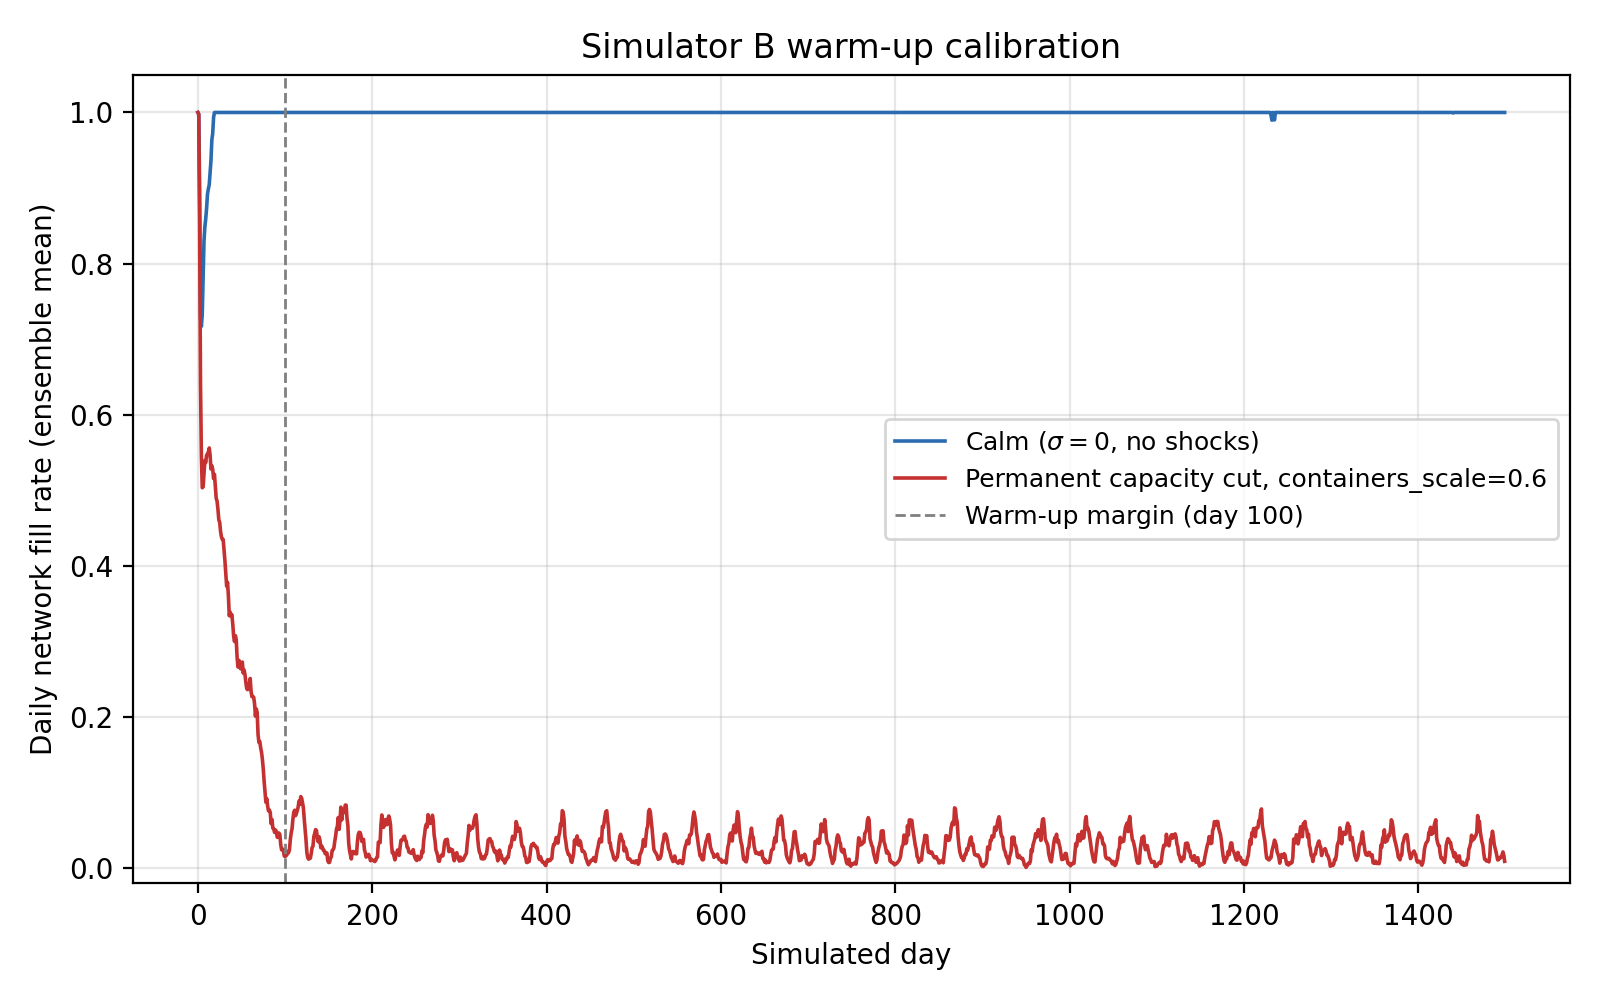
\includegraphics[width=0.72\textwidth]{warmup_figure.png}
\caption{Simulator B warm-up check on the patched simulator: 5-seed ensemble-mean daily fill rate over a 1{,}500-day pilot horizon, calm vs.\ a permanent \texttt{containers\_scale}=0.6 capacity cut. The calm regime stabilizes by $\sim$day 100, fixing the warm-up margin used to size $L$; the permanent-cut regime instead settles into a severely degraded new equilibrium only after $\sim$600--700 days --- exactly the pathology bounded, timed disruptions are designed to avoid, per the design-rationale note below.}
\label{fig:warmup}
\end{figure}

\paragraph{A scheduled-capacity patch (patch 3): timed, graded disruptions.} \texttt{containers\_scale} (patch 2 and the design-rationale note below) rescales capacity once, permanently, at network construction --- the right mechanism for characterizing a stability boundary, the wrong one for a bounded disruption-and-recovery event. The simulator already computes a per-day \texttt{capacity\_factor} inside its daily reset call (\texttt{reset\_daily\_edges}), currently hardcoded to 1.0 every day; patch 3 replaces that hardcoded value with a day-dependent one --- the severity-mapped scale during $[T_0, T_0+D)$, and 1.0 outside it --- reusing an existing hook rather than adding new machinery, and is a no-op whenever the disruption window is empty, matching the pattern of patches 1--2. This patch, not the platform's own targeted-edge-cut extension, is what the timed disruptions in Table~\ref{tab:shift} are built on; the extension was checked and rejected for this role (Simulator B description, Section~\ref{sec:architecture}).

\paragraph{Severity on B is overload $\nu$, not a capacity fraction (v12).} A scan of 11 capacity levels $\times$ 3 durations (Gate~4) showed that the earlier mapping $c=1-0.75\sigma$ makes the Mild band ($\sigma\leq0.2$, $c\geq0.85$) a calm-weather band: the last-mile tier carries $\approx1.29\times$ nominal demand, so a cut to $c\geq0.775$ loses nothing and training data there would carry no disruption signal. Severity on B is therefore defined by \emph{overload} $\nu=\max(0,\,1-1.29\,c)$, the share of demand the network cannot carry during the event. Recovery time then follows $\text{TTR}\approx k\,D\,\nu/0.29$ with $k=1.07$ ($R^2=0.95$, 63 uncensored runs). Bands: Mild $0<\nu\leq0.15$ (training; $D\in\{14,30\}$), Moderate $0.15$--$0.35$, Severe $0.35$--$0.55$, Extreme $0.55$--$0.68$ (test). Fill rate floors at zero in severe cells, so \emph{unmet demand} (days of demand lost over the post-warm-up window) is the primary B metric and fill rate secondary; the practical margin $\delta=0.5$ percentage points of fill rate corresponds to $1.5$ days of unmet demand at $L=400$. On B the policy is a $5\times5$ grid of safety-stock scale $\times$ pipeline multiplier; five of the 25 are not viable even in calm weather (calm fill $<0.99$; Gate~3) and are dropped, leaving 20 policies (190 pairs). Calm-only training is kept as an ablation arm. Gates~5--6 (1{,}800 runs, 5 seeds per cell) confirm the Mild band carries real disruption (mean unmet demand $1.1$--$11.1$ days; $82$--$100\%$ of runs lose demand), that the median share of decidable policy pairs is $0.86$ (cells with real loss), that random policy advice costs more than $\delta$ in all 17 such cells, and that the minimum detectable difference falls from $1.8$ to $0.7$ days between 5 and 30 seeds. Disruptions in B are timed capacity cuts only, so protocol P2 (type transfer) is Simulator-A-only.

\paragraph{Pilot learnability check (v12).} Before collecting training data, four surrogate families (quadratic ridge, random forest, gradient boosting, neural net) were fitted to the Mild-band pilot runs and scored on held-out seeds, then on cells outside the band. In-band all four reach the seed-noise ceiling ($R^2=0.64$--$0.65$ against a ceiling of $0.65$) and rank policies near-perfectly (Spearman $\geq0.96$), but the best policy is nearly constant across Mild cells, so in-band regret cannot separate surrogates from a fixed rule. Outside the band, mean regret rises from $\approx0.02$ to $\approx4$ days, no better than a constant policy: the shift effect the study is built to measure is present in pilot data. These are 5-seed, 600-run pilot numbers and are not reported as results.

\paragraph{Design rationale: why timed disruptions, not permanent regime settings.} The reason is a stability boundary discovered while characterizing \texttt{containers\_scale} as a permanent knob, reported in full in a companion technical note and stated here only as the conclusion that motivates the main design. Because last-mile capacity on this network self-calibrates to $(\text{target\_ratio}/\text{packing\_eff}) \times \text{containers\_scale} \approx 1.290 \times \text{containers\_scale}$ times demand, a permanent capacity cut has a theoretical stability threshold at $\text{containers\_scale}^{*} = \text{packing\_eff}/\text{target\_ratio} \approx 0.775$, below which demand permanently exceeds capacity. An empirical characterization (5 seeds, seven \texttt{containers\_scale} values, horizons of 800--3{,}000 days; Figure~\ref{fig:stability}) confirms a three-tier structure: $\geq$0.80 is robustly stable (relaxation time $\tau\approx553$ days); $\leq$0.70 is robustly unstable (backlog growth never decays); the interval $(0.75, 0.80)$ shows \emph{critical slowing down} \citep{whitt2002} rather than resolving cleanly either way at any practical horizon. Below the threshold, all $(s,S)$ policies converge to near-identical throughput --- capacity, not policy, becomes the binding constraint --- so policy comparisons there are structurally degenerate regardless of how long they run. Bounded, timed disruptions sidestep this: a severe-but-temporary event still differentiates policies on how much damage accumulates and how fast the system recovers, long after a permanent-regime comparison at the same severity would have gone degenerate. This finding neither appears in nor contradicts the original ISOMORPH paper --- Appendix B.4 of \citet{zhang2026isomorph} restricts all reported evaluation to demand-side knobs, excluding \texttt{containers\_scale} entirely --- it is a property of the simulator their forecasting-focused evaluation had no reason to examine.

\begin{figure}[H]
\centering
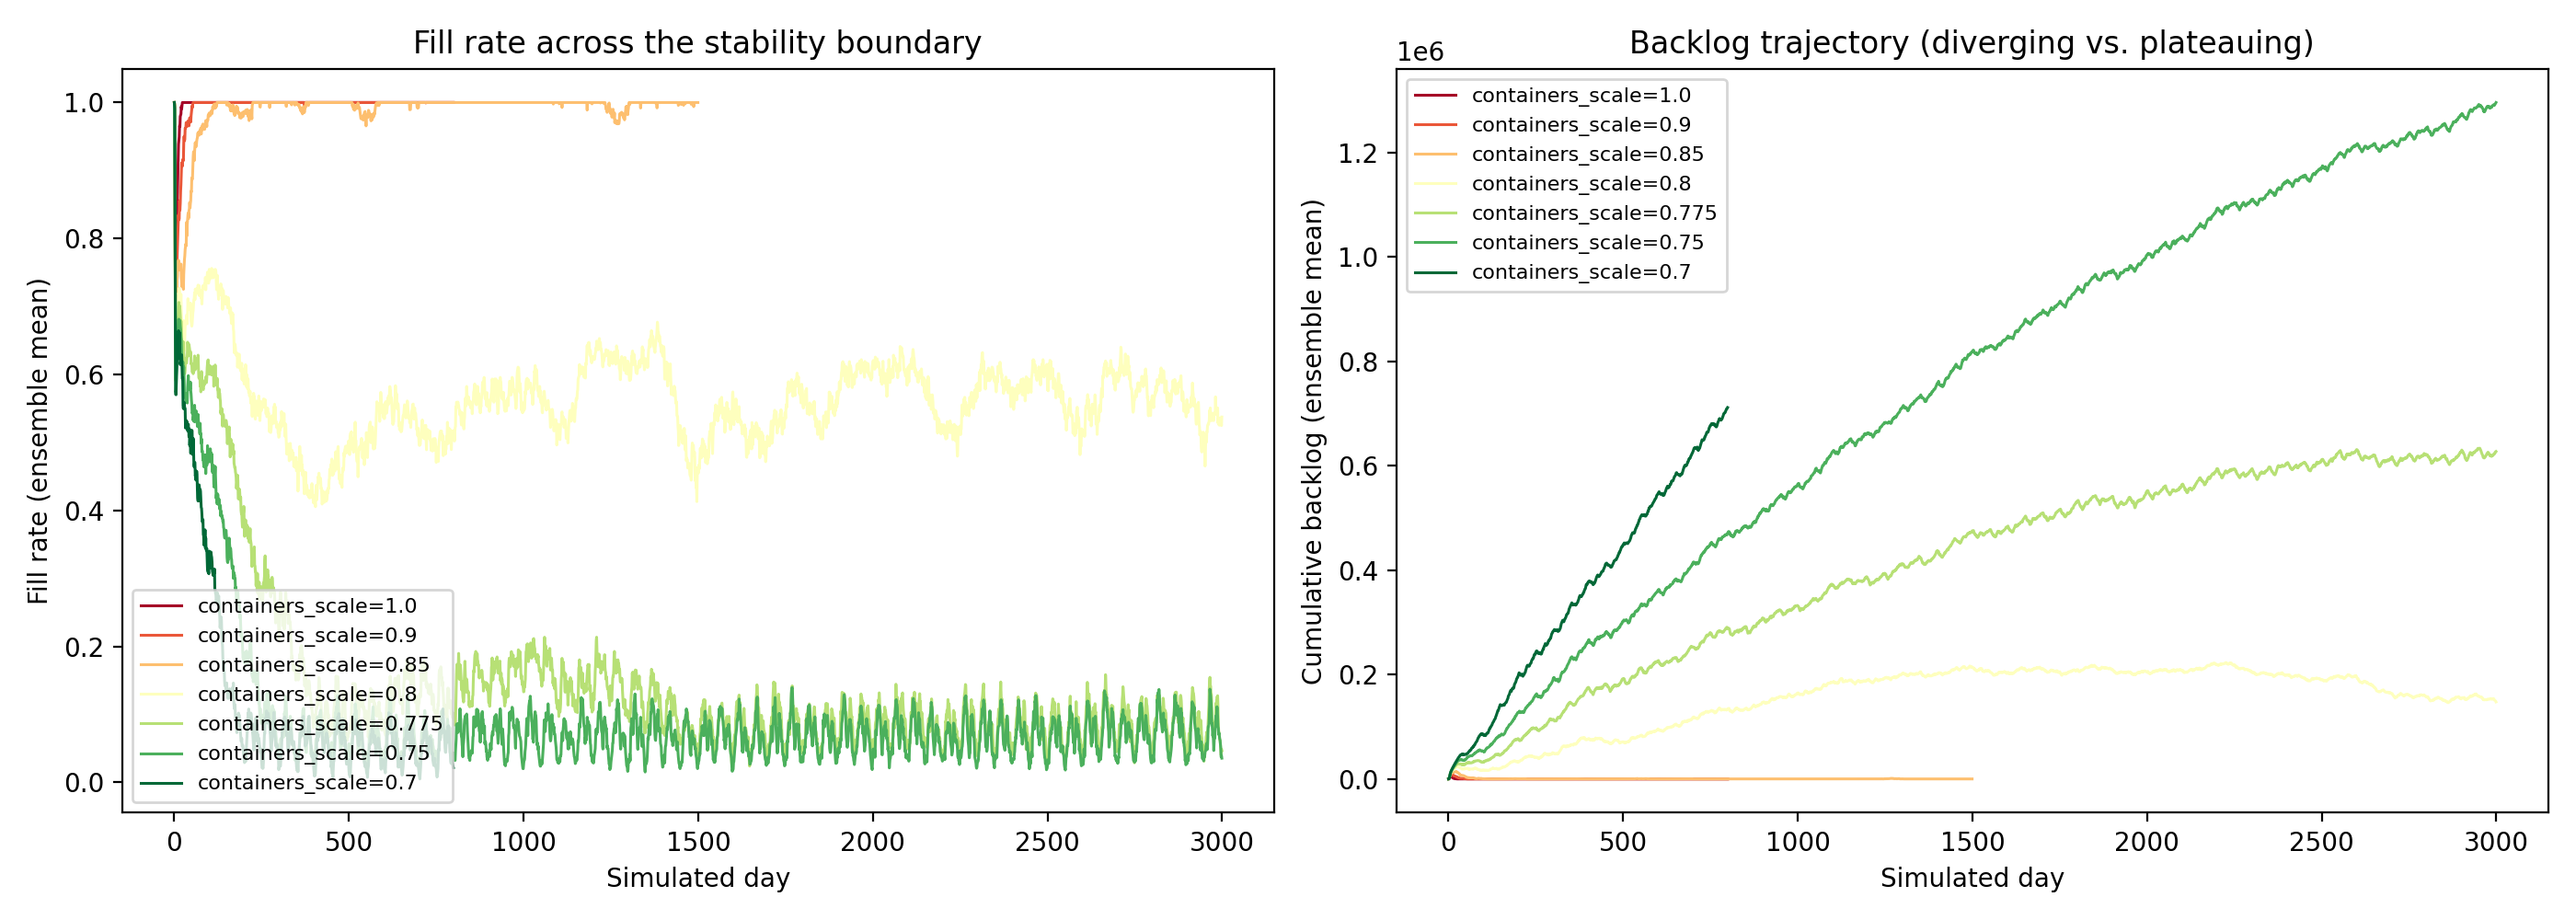
\includegraphics[width=0.95\textwidth]{stability_boundary_figure.png}
\caption{Stability-boundary characterization under permanent \texttt{containers\_scale} settings (5-seed ensemble means, shock-free demand; full derivation in the companion note). Left: fill rate; right: cumulative backlog. $\texttt{containers\_scale}\geq0.80$ (green) converges to a stable equilibrium; $\leq$0.75 (orange/red) shows sustained or accelerating backlog growth. This is the design rationale for using timed rather than permanent disruptions in the main study.}
\label{fig:stability}
\end{figure}

Both simulators' training-generation runs are independent processes and parallelize directly across cores; both are generated as idempotent, checkpointed jobs, so a full grid never depends on one unbroken session.

% ============================================================
\section{Experimental Design Summary}
% ============================================================

\begin{table}[H]
\centering
\caption{Factor grid (Simulator A; B uses its native knobs)}
\label{tab:factors}
\footnotesize
\begin{tabular}{p{4.6cm}p{9.0cm}}
\toprule
\textbf{Factor} & \textbf{Range} \\
\midrule
Disruption severity $\sigma$ & $[0,1]$ in bins $\{0,\,0.1,\,\ldots,\,1.0\}$ \\
Disruption duration $D$ & short / medium / long ($\sim$14 / 30 / 90 days) \\
Shock type & demand surge / capacity loss / lead-time inflation / compound \\
 $(s,S)$ grid & 5$\times$5 factor levels spanning lean$\rightarrow$buffered: 25 policies, 300 pairs, one family \\
 Dual/option-sourcing & binary choice, kept as a second family crossed onto the 25 $(s,S)$ policies (50 policies, 1{,}225 pairs) rather than pooled into one, so multiplicity correction is not diluted across two structurally different comparisons \\
Demand variability & low / medium / high \\
Lead-time variability & low / high \\
Seeds & 30 per design point (paired across policies; deepened for near-ties) \\
Decidability & practical margin $\delta$; BH FDR $q=0.10$ within severity $\times$ duration $\times$ shock-type families, computed separately per policy family above \\
\bottomrule
\end{tabular}
\end{table}

\begin{table}[H]
\centering
\caption{Regime definitions (training-eligible regimes in bold)}
\label{tab:regimes}
\footnotesize
\begin{tabular}{llp{8.2cm}}
\toprule
\textbf{Regime} & $\sigma$ (A) / $\nu$ (B, v12) & \textbf{Interpretation} \\
\midrule
\textbf{Calm} & 0 & Baseline operations (\textbf{training}) \\
\textbf{Mild} & 0--0.2 / 0--0.15 & Absorbable perturbations (\textbf{training}); on B, $\nu>0$ so the event actually removes capacity below demand \\
Moderate & 0.2--0.5 & Queueing pressure visible (test only) \\
Severe & 0.5--0.8 & Backlog accumulation; policy-sensitive region \\
Extreme & 0.8--1.0 & Near-collapse dynamics \\
\bottomrule
\end{tabular}
\end{table}

\begin{table}[H]
\centering
\caption{Duration levels, crossed independently with severity (training-eligible levels in bold)}
\label{tab:duration}
\footnotesize
\begin{tabular}{llp{8.2cm}}
\toprule
\textbf{Level} & $D$ (days) & \textbf{Interpretation} \\
\midrule
\textbf{Short} & $\sim$14 & Comparable to a single reorder cycle (\textbf{training}) \\
\textbf{Medium} & $\sim$30 & A few reorder cycles (\textbf{training}) \\
Long & $\sim$90 & Comparable to or exceeding several nodes' replenishment lead times; policy-timing effects (H5) expected here (test only) \\
\bottomrule
\end{tabular}
\end{table}

% ============================================================
\section{Expected Results and Interpretation}\label{sec:results}
% ============================================================

The interpretation rules below are pre-specified to prevent post-hoc rationalization. They are \emph{not} claims that all outcomes are equally valuable: the validation's scientific weight depends on which branch occurs, and the weakest branch (universal robustness) is explicitly acknowledged as such --- it would likely warrant a shorter protocol/benchmark paper rather than a full-length article, and the project accepts that risk upfront.

\begin{table}[H]
\centering
\caption{Pre-specified interpretation rules}
\label{tab:tree}
\footnotesize
\begin{tabular}{p{6.0cm}p{4.2cm}p{3.9cm}}
\toprule
\textbf{Outcome} & \textbf{Meaning} & \textbf{Framing} \\
\midrule
Large excess-over-placebo regret + rank flips at high $\sigma$; $\Delta(\sigma)$ grows & Fast copies mislead precisely in severe disruptions & Warning paper; the field's adoption is ahead of its evidence \\
\midrule
Regret concentrated in specific model classes or output types & Practical selection guidance (which surrogate, which output, how far) & Protocol + guidance paper \\
\midrule
Regret negligible and coverage holds across regimes & First trust certification for twin-style scenario testing & Standardization contribution; expected to be the least eventful branch, targeted at a venue that values benchmarks and protocols \\
\midrule
 $DR$ uncorrelated with prediction error (H4) & Accuracy metrics are the wrong instrument for twin reliability & Evaluation-theory contribution \\
\bottomrule
\end{tabular}
\end{table}

% ============================================================
\section{Contributions}
% ============================================================

\begin{enumerate}
\item \textbf{The validation.} First systematic decision-reliability assessment of ML surrogates of supply-chain simulators under disruption-regime shift, replicated across two independent platforms --- answering, with evidence, the validity question the 2026 literature poses in print \citep{ivanov2026,liu2026,huang2026,soykan2026}.
\item \textbf{The protocol.} A reusable, open evaluation suite (shift protocols; decision-regret definition for simulator surrogates; \emph{noise-aware, multiplicity-controlled ranking-stability diagnostics with a placebo noise floor}; coverage-deficit curves) that subsequent digital-twin and surrogate papers can adopt as standard reporting practice.
\item \textbf{The verdict.} Operational guidance: below which severity, and for which output types, twin-style scenario testing can be trusted --- and where it must be replaced by full simulation.
\end{enumerate}

\subsection{What is technically new (anticipating the assembly question)}

Because the contribution is explicitly \emph{transfer and application}, a referee or committee member will reasonably ask what is new beyond assembly. Three elements are technical contributions in themselves: (i) the \emph{noise-aware flip criterion} --- combining common-random-number paired evaluation \citep{law2015}, a decidable-pair rule with a pre-registered practical margin and Benjamini--Hochberg false-discovery-rate control across the pairwise family \citep{benjamini1995,benjamini2001}, and a placebo noise floor --- without which ranking-stability claims in stochastic simulation are confounded first by Monte Carlo noise and then by multiplicity (we are not aware of an existing surrogate validation that applies this discipline); (ii) the \emph{regime-shift protocols} adapted to DES, where shift is abrupt, multi-modal, and state-accumulating rather than smooth covariate drift; (iii) the \emph{coverage-deficit curve} quantifying conformal-reliability degradation as a function of disruption severity. The validation object and its verdict are the conceptual contributions; these three are the methodological ones.

% ============================================================
\section{Scope, Assumptions, and Honesty Guards}
% ============================================================

\begin{itemize}
\item \textbf{Synthetic data only, by design.} The claims are about the reliability of a method \emph{class}, not about any real firm or corridor. Synthetic evidence is the legitimate standard for methodological validation studies; no real-world causal or descriptive claims are made.
\item \textbf{No metric novelty claimed.} Conformal prediction \citep{vovk2005,angelopoulos2023,tibshirani2019}, decision regret \citep{elmachtoub2022,ban2019}, FDR control \citep{benjamini1995,benjamini2001}, and shift testing are imported and cited. The claim is transfer, adaptation, and first systematic application to this object; the genuinely technical elements are itemized in Section~7.1.
\item \textbf{Terminology discipline.} The phrase ``digital twin'' is used only to situate the object (the simulation/ML core of twin architectures) \citep{ivanov2021,meliani2026}; no live-data twin is claimed or required.
\item \textbf{Verifiable claims.} ``First''/``no study'' statements are backed by a documented four-direction search log; final forward-citation re-check before submission.
\item \textbf{Preprint dependence.} ISOMORPH \citep{zhang2026isomorph} and the nearest working papers \citep{li2026ssrn,acuna2026} are preprints. The two-simulator architecture ensures the paper does not stand on any single unreviewed artifact.
\item \textbf{Fixed boundary.} No reinforcement learning, no adaptive sampling, no new surrogate architectures, no real-data case study. Any of these is future work; each would convert a lean validation into a multi-year project.
\end{itemize}

% ============================================================
\section{Risks and Mitigation}
% ============================================================

\begin{table}[H]
\centering
\caption{Risks and mitigation}
\label{tab:risks}
\footnotesize
\begin{tabular}{p{4.6cm}p{9.6cm}}
\toprule
\textbf{Risk} & \textbf{Mitigation} \\
\midrule
Simulator A dismissed as ``toy'' & Transparency + verification tests \citep{law2015}; replication on independent platform B; protocol released so others can validate their own simulators \\
\midrule
Near-tie policies or test multiplicity inflate apparent rank flips (noise masquerading as surrogate failure, at either level) & Practical-margin decidability + BH FDR control within families + common random numbers + placebo noise floor + adaptive deepening with recomputed correction (Section~\ref{sec:metrics}); undecidable mass reported explicitly \\
\midrule
ISOMORPH friction (API, immaturity, a released horizon far too slow for the full grid at laptop scale, a shock generator whose density is horizon-dependent, and a capacity knob confounded by integer rounding and self-calibration ordering; the platform's own targeted-edge-cut extension cannot substitute for timed disruptions, being both non-functional and binary-depth) & Simulator A is primary and self-contained; B is a replication column, not a dependency; addressed by three disclosed, single-purpose patches (all no-ops at released defaults) --- horizon-independent shock duration, permanent capacity rescaling, and a scheduled per-day capacity factor for timed disruptions (Section~\ref{sec:compute}) --- a uniform, pilot-calibrated run length $L=400$ days applied identically to training and test, an empirically characterized permanent-regime stability boundary at \texttt{containers\_scale}$\in(0.75,0.80)$ retained as the design rationale for using timed disruptions rather than a target to hit in the main experiment, and parallel, checkpointed execution to keep wall-clock time well below the CPU-hour total \\
\midrule
Scoop risk (adjacent working-paper authors extend toward the validation) & Lean design; working paper within months of results; monitoring of the relevant repositories and author pages \\
\midrule
``Conformal fails under shift'' is trivially true & Even so, the quantified deficit curve is new for this setting; weighted-conformal repair \citep{tibshirani2019} adds methodological content \\
\midrule
Surrogates turn out robust & Trust-certification result (Table~\ref{tab:tree}); acknowledged as the weakest branch --- reframed as a benchmark/protocol paper if it occurs \\
\midrule
Compute or scope overrun & Fixed boundary (Section~9); factorial grids pruned by screening; every headline result exists at 1/10 scale before full grids are run \\
\bottomrule
\end{tabular}
\end{table}

% ============================================================
\section{Reproducibility}
% ============================================================

Fixed seeds; versioned configuration files; one-script regeneration of every table and figure; surrogate-provenance record linking each trained model to its exact training slice; the placebo pipeline, the decidable-pair logic, and the FDR correction are part of the released code, so every flip count and its full error budget can be independently recomputed; public release of code, configurations, and run datasets under an open license (Simulator A: original code; Simulator B: MIT as released \citep{zhang2026isomorph}). Conformal calibration implemented on standard tooling.\footnote{\url{https://github.com/scikit-learn-contrib/MAPIE}}

% ============================================================
\section*{References}
\addcontentsline{toc}{section}{References}
% ============================================================

\begin{thebibliography}{99}

\bibitem[Acu\~na(2026)]{acuna2026} Acu\~na, J.J.S. (2026). A calibration-aware reference architecture for resilient supply chain planning: integrating conformal probabilistic demand forecasting with scenario-based planning. \textit{Research Square} (preprint).

\bibitem[Aldridge(2026)]{aldridge2026} Aldridge, I. (2026). Regret equals covariance: a closed-form characterization for stochastic optimization. \textit{arXiv preprint} arXiv:2605.14019.

\bibitem[Angelopoulos and Bates(2023)]{angelopoulos2023} Angelopoulos, A.N., \& Bates, S. (2023). Conformal prediction: a gentle introduction. \textit{Foundations and Trends in Machine Learning}, 16(4), 494--591.

\bibitem[Ban and Rudin(2019)]{ban2019} Ban, G.-Y., \& Rudin, C. (2019). The big data newsvendor: practical insights from machine learning. \textit{Management Science}, 65(1), 87--103.

\bibitem[Benjamini and Hochberg(1995)]{benjamini1995} Benjamini, Y., \& Hochberg, Y. (1995). Controlling the false discovery rate: a practical and powerful approach to multiple testing. \textit{Journal of the Royal Statistical Society: Series B}, 57(1), 289--300.

\bibitem[Benjamini and Yekutieli(2001)]{benjamini2001} Benjamini, Y., \& Yekutieli, D. (2001). The control of the false discovery rate in multiple testing under dependency. \textit{Annals of Statistics}, 29(4), 1165--1188.

\bibitem[Breiman(2001)]{breiman2001} Breiman, L. (2001). Random forests. \textit{Machine Learning}, 45(1), 5--32.

\bibitem[Bruneau et al.(2003)]{bruneau2003} Bruneau, M., Chang, S.E., Eguchi, R.T., Lee, G.C., O'Rourke, T.D., Reinhorn, A.M., Shinozuka, M., Tierney, K., Wallace, W.A., \& von Winterfeldt, D. (2003). A framework to quantitatively assess and enhance the seismic resilience of communities. \textit{Earthquake Spectra}, 19(4), 733--752.

\bibitem[Charoenwut and Kulvatunyou(2026)]{charoenwut2026} Charoenwut, P., Kulvatunyou, B., et al. (2026). Opportunities and gaps in supply chain digital twin deployments: a biopharmaceutical industry focus. \textit{ASME Journal of Computing and Information Science in Engineering}.

\bibitem[Chen and Guestrin(2016)]{chen2016} Chen, T., \& Guestrin, C. (2016). XGBoost: a scalable tree boosting system. In \textit{Proceedings of the 22nd ACM SIGKDD Conference}, 785--794.

\bibitem[Elmachtoub and Grigas(2022)]{elmachtoub2022} Elmachtoub, A.N., \& Grigas, P. (2022). Smart ``predict, then optimize''. \textit{Management Science}, 68(1), 9--26.

\bibitem[Fan et al.(2026)]{fan2026} Fan, C., Lai, J., Xiao, F., Wang, Z., \& Mo, J. (2026). Right where it matters: a decision-focused end-to-end learning method for enhanced building energy flexibility. \textit{Advances in Applied Energy}.

\bibitem[Gopakumar et al.(2026)]{gopakumar2026} Gopakumar, V., Gray, A., Oskarsson, J., et al. (2026). Uncertainty quantification of surrogate models using conformal prediction. \textit{Machine Learning: Science and Technology}.

\bibitem[Giannopoulos et al.(2026)]{giannopoulos2026} Giannopoulos, P.G., Malamas, V., et al. (2026). Inventory management decision-making under zero-knowledge conditions: a behavioral cloning approach. \textit{SSRN} (preprint).

\bibitem[Holm(1979)]{holm1979} Holm, S. (1979). A simple sequentially rejective multiple test procedure. \textit{Scandinavian Journal of Statistics}, 6(2), 65--70.

\bibitem[Henry and Ramirez-Marquez(2012)]{henry2012} Henry, D., \& Ramirez-Marquez, J.E. (2012). Generic metrics and quantitative approaches for system resilience as a function of time. \textit{Reliability Engineering and System Safety}, 99, 114--122.

\bibitem[Hosseini et al.(2019)]{hosseini2019} Hosseini, S., Ivanov, D., \& Dolgui, A. (2019). Review of quantitative methods for supply chain resilience analysis. \textit{Transportation Research Part E}, 125, 285--307.

\bibitem[Huang et al.(2026)]{huang2026} Huang, Y., Ghadge, A., \& Yates, N. (2026). Impact of digital twin adoption on food supply chain performance: a system dynamics approach. \textit{International Journal of Production Research}.

\bibitem[Im et al.(2026)]{im2026} Im, H., Benslimane, W., \& Grigas, P. (2026). Smart surrogate losses for contextual stochastic linear optimization with robust constraints. \textit{Advances in Neural Information Processing Systems (NeurIPS)}.

\bibitem[Ivanov and Dolgui(2021)]{ivanov2021} Ivanov, D., \& Dolgui, A. (2021). A digital supply chain twin for managing the disruption risks and resilience in the era of Industry 4.0. \textit{Production Planning \& Control}, 32(9), 775--788.

\bibitem[Ivanov(2026)]{ivanov2026} Ivanov, D. (2026). Agentic digital twins: bridging model-based and AI-driven decision-making support for a new era of supply chain and operations management. \textit{International Journal of Production Research}.

\bibitem[Kaiyrkhan(2026)]{kaiyrkhan2026} Kaiyrkhan, N. (2026). Decision-focused stochastic optimization for AI-driven pharmaceutical supply chains. \textit{Proceedings of the 6th IEEE International Conference}.

\bibitem[Kleijnen(2015)]{kleijnen2015} Kleijnen, J.P.C. (2015). \textit{Design and Analysis of Simulation Experiments} (2nd ed.). Springer.

\bibitem[Law(2015)]{law2015} Law, A.M. (2015). \textit{Simulation Modeling and Analysis} (5th ed.). McGraw-Hill.

\bibitem[Lee et al.(1997)]{lee1997} Lee, H.L., Padmanabhan, V., \& Whang, S. (1997). Information distortion in a supply chain: the bullwhip effect. \textit{Management Science}, 43(4), 546--558.

\bibitem[Li(2026a)]{li2026ssrn} Li, P. (2026). Forecasting for inventory decisions: a decision-regret benchmark for perishability-aware multi-echelon retail replenishment using the M5/Walmart data. \textit{SSRN} 7051299 (preprint).

\bibitem[Li et al.(2026b)]{libranke2026} Li, X., Branke, J., \& Doan, X.V. (2026). How much data do we need? Sequential data collection for stochastic programming. \textit{arXiv preprint} arXiv:2607.10207.

\bibitem[Liu et al.(2026)]{liu2026} Liu, C., Wang, Y., Purvis, L., \& Potter, A. (2026). Can digital twin Technology enhance supply-chain resilience? A systematic literature review. \textit{Sustainability}.

\bibitem[Meliani and Sahin(2026)]{meliani2026} Meliani, Y., \& Sahin, E. (2026). Towards scalable supply chain digital twins: a review and maturity assessment framework. \textit{Journal of Logistics Research and Applications}.

\bibitem[Mi\v{s}i\'{c} and Perakis(2020)]{misic2020} Mi\v{s}i\'{c}, V.V., \& Perakis, G. (2020). Data analytics in operations management: a review of recent research. \textit{Manufacturing \& Service Operations Management}, 22(4), 930--947.

\bibitem[Mukherjee et al.(2026)]{mukherjee2026} Mukherjee, S., Pham, A.D., Pibernik, R., \& Xu, Y. (2026). In-context learning for data-driven censored inventory control. \textit{arXiv preprint}.

\bibitem[Qiao et al.(2026)]{qiao2026} Qiao, T., Eckman, D.J., \& Nelson, B.L. (2026). Plausible intervals: global inference from limited simulation of structured problems. \textit{ACM Transactions on Modeling and Computer Simulation}.

\bibitem[Rasmussen and Williams(2006)]{rasmussen2006} Rasmussen, C.E., \& Williams, C.K.I. (2006). \textit{Gaussian Processes for Machine Learning}. MIT Press.

\bibitem[Sacks et al.(1989)]{sacks1989} Sacks, J., Welch, W.J., Mitchell, T.J., \& Wynn, H.P. (1989). Design and analysis of computer experiments. \textit{Statistical Science}, 4(4), 409--423.

\bibitem[Scalese et al.(2026)]{scalese2026} Scalese, A., Narayanan, S., \& Antoniou, C. (2026). GUIDED: network-agnostic feature initialization for spatial transferability in GNN-based models. \textit{arXiv preprint} arXiv:2607.19270.

\bibitem[Shen(2026)]{shen2026} Shen, Y. (2026). When do surrogate updates improve decisions? A local theory of trajectory-wise transfer. \textit{arXiv preprint} arXiv:2608.01130.

\bibitem[Soykan and Rabadi(2026)]{soykan2026} Soykan, B., \& Rabadi, G. (2026). Integrating AI and ML in supply chain digital twins. In: \textit{Optimizing Supply Chains Through Digital Twins} (edited volume).

\bibitem[Tibshirani et al.(2019)]{tibshirani2019} Tibshirani, R.J., Barber, R.F., Cand\`es, E., \& Ramdas, A. (2019). Conformal prediction under covariate shift. \textit{Advances in Neural Information Processing Systems (NeurIPS)}.

\bibitem[Tolia and Ponis(2026)]{tolia2026} Tolia, A., \& Ponis, S.T. (2026). Digital twins for real-time decision-making in supply chain management and logistics: a systematic review. \textit{Information}.

\bibitem[Vovk et al.(2005)]{vovk2005} Vovk, V., Gammerman, A., \& Shafer, G. (2005). \textit{Algorithmic Learning in a Random World}. Springer.

\bibitem[Whitt(2002)]{whitt2002} Whitt, W. (2002). \textit{Stochastic-Process Limits: An Introduction to Stochastic-Process Limits and Their Application to Queues}. Springer Series in Operations Research. Springer.

\bibitem[Zhang et al.(2026)]{zhang2026isomorph} Zhang, Z., Gu, H., Zhang, B.J., Elenius, D., Tyrrell, M., et al. (2026). ISOMORPH: a supply chain digital twin for simulation, dataset generation, and forecasting benchmarks. \textit{arXiv preprint}.

\bibitem[Zimmel et al.(2026)]{zimmel2026} Zimmel, A., Setinek, P., Galletti, G., Brandstetter, J., et al. (2026). Stabilizing test-time adaptation of high-dimensional simulation surrogates via D-optimal statistics. \textit{arXiv preprint}.

\end{thebibliography}

\vspace{0.3cm}
\noindent\textit{Note: several 2026 items are preprints; bibliographic metadata (arXiv IDs, DOIs, final venues) will be verified and updated before any submission. \textbf{Version 3 changes:} multiplicity control (BH FDR $q=0.10$ within severity $\times$ shock-type families; Holm sensitivity), practical-margin decidability ($\delta$), placebo-noise-floor integration with the FDR bound, BH recomputation after adaptive deepening, and matching updates to RQ2, H2, contributions, risk table, and reproducibility. \textbf{Version 4 changes:} empirical benchmark of Simulator B's baseline runtime (409.9\,s per 20-year rollout, released configuration), retraction of the ``B is vectorized and faster'' claim, a horizon-truncation compute plan for B with a worked before/after estimate, clarification that ISOMORPH's released sweeps calibrate rather than supply the regret-pipeline data, a noted stretch-goal extension of P3 to Simulator B via its targeted edge-cut knobs, and a stale cross-reference fix in the risk table. \textbf{Version 5 changes:} disclosure of a one-line, no-op-at-7{,}300-days patch to ISOMORPH's shock generator (duration scaled to requested horizon); a pilot warm-up study (5 seeds, calm vs.\ capacity-cut, 1{,}500-day horizon) fixing the production horizon at 700 days, with Figure~\ref{fig:warmup}; the corrected compute estimate ($\approx$22--27 CPU-hours for B's training runs, superseding the earlier untested $\sim$150-day/6-hour guess); and a flagged recalibration need for the severity-to-\texttt{containers\_scale} mapping given the network's thin capacity margin. \textbf{Version 6 changes:} correction of an error in v5, which applied the 700-day severe-regime horizon to the training runs as well; training data (restricted to $\sigma \leq 0.2$) now uses a 200-day horizon matched to the calm/mild stabilization point in Figure~\ref{fig:warmup}, cutting the training-run budget from $\approx$22--27 to $\approx$7--8 CPU-hours; the 700-day horizon is reserved for the severe-range test grid; and an explicit parallel, checkpointed execution plan is added, converting CPU-hour totals into realistic wall-clock estimates (e.g., $\approx$2 hours at 4 workers) and removing the need for one unbroken run. \textbf{Version 7 changes:} disclosure of a second ISOMORPH patch (capacity scaling moved from an integer container count to the continuous \texttt{container\_volume} field, applied after last-mile self-calibration, no-op at \texttt{containers\_scale}=1.0); an analytically derived and empirically confirmed stability boundary at \texttt{containers\_scale}$\in(0.75,0.80)$, characterized as an interval rather than a point due to critical slowing down \citep{whitt2002}, with Figure~\ref{fig:stability}; a revised severity mapping for Mild training data ($\text{containers\_scale}=1-0.75\sigma$) keeping it clear of the critical band; and an explicit statement that this finding is absent from, not contradicted by, the original ISOMORPH evaluation. \textbf{Version 8 changes:} title updated to ``Can We Trust the Fast Copy? A Decision-Regret Validation of Machine-Learning Surrogates of Supply-Chain Simulators Under Disruption''; H5 pre-registered (regret non-monotone in severity, peaking near the stability boundary, per Figure~\ref{fig:stability}); ``two open simulators'' corrected to ``one open platform, one disclosed modified fork''; ``defect'' retired in favor of ``limitation'' for the capacity/self-calibration issue specifically (the duration-generator issue keeps its bug-like framing, since it is one relative to the tool's own stated design); the released sweep's five discrete achievable capacity levels (1, 2, 3, 4, 8 containers) stated explicitly as consistent with categorical-scenario design intent; \texttt{giannopoulos2026} now cited in the DFL landscape row rather than sitting unused in the bibliography; and the hardcoded ``Section~5.6'' cross-reference replaced with a proper label. \textbf{Open from external review, not yet incorporated:} the train/test evaluation-window definition (fixed post-warm-up window vs.\ whole-run average) flagged as a possible confound; Simulator A's own warm-up study, cost-layer coefficients, and $\delta$ justification; a documented search-log artifact; the H4 test statistic (block-bootstrapped Spearman); the protocol$\,\times\,$simulator matrix; and moving implementation-forensic detail to an appendix. These are substantive enough to need their own pass rather than a terminology sweep. \textbf{Version 9 changes:} full terminology sweep, ``audit''$\,\to\,$``validation'' (28 instances: header, cover box, elevator pitch, landscape table, nearest-neighbours discussion, novelty claim, Simulator B/decision-layer prose, risk table, contributions, scope/assumptions, reproducibility), now consistent with the title changed in v8; the literature-tracking log specifically disambiguated as the ``search log'' throughout, distinct from ``the validation'' (the study itself); internal section labels left unchanged (invisible to readers). \textbf{Version 10 changes:} switched the core experimental design from permanent regime-shift severity to timed, bounded-duration disruptions ($\sigma$ and $D\in\{\text{short,medium,long}\}\approx\{14,30,90\}$ days), per external review; added a third disclosed patch (scheduled per-day capacity factor via an existing, previously-hardcoded simulator hook) after confirming the platform's own targeted-edge-cut extension cannot serve this role (non-functional import error, and binary-depth even if it could run); replaced the 200/700-day split with one uniform, pilot-calibrated run length $L\approx300$ days applied identically to training and test, resolving the train/test evaluation-window confound flagged in external review; added window-limited primary metrics (cumulative unmet demand, resilience-triangle area, peak backlog) and censored time-to-recovery as a secondary metric, citing \citet{bruneau2003} and \citet{henry2012}; repurposed the permanent-regime stability-boundary finding as the design rationale for the timed-disruption choice rather than the main experiment's mechanism, with full derivation pointed to a companion technical note; rewrote H5 as a two-dimensional, non-monotone-in-$(\sigma,D)$ hypothesis naming two candidate mechanisms (lead-time mismatch; recoverability edge) without pre-committing between them, and operationalized H2 with the leave-one-output-true ablation it was missing; added Simulator A's own warm-up pilot as a validation-protocol step; resolved the H4 pair-count inconsistency (300 vs.\ 1{,}225) with two separate policy families rather than pooling them; added a duration table (Table~\ref{tab:duration}) crossed independently with the existing severity table. \textbf{Still open:} Simulator A's cost-layer coefficients and $\delta$ justification; the H4 test statistic (block-bootstrapped Spearman); the search-log artifact; moving implementation-forensic detail --- including this changelog, now long enough to be a symptom of the concern itself --- to an appendix at manuscript stage. \textbf{Version 11 changes:} documented \texttt{pipeline\_mult=7} (Section~\ref{sec:compute}) --- confirmed dynamic (drives the daily shipping target, not computational) and confirmed matched to ISOMORPH's own released baseline configuration (built-in default is 0), per external review; this changelog is now long enough to be doing real harm to the document's readability and is a standing candidate for compression whenever the appendix migration happens, not just a relocation target. \textbf{Version 12 changes:} severity on Simulator B redefined as capacity overload $\nu=\max(0,1-1.29c)$ after Gate~4 showed the earlier Mild band loses no demand; run length raised from $L\approx300$ to $L=400$ (compute re-estimated); unmet demand adopted as primary B metric because fill rate floors at zero; policy grid on B fixed at 20 viable $(\text{safety-stock},\text{pipeline})$ policies after Gate~3; Gates~5--6 and a pilot surrogate-learnability check reported; calm-only training added as an ablation arm; P2 flagged as A-only; figure paths moved to the repository. \textbf{Still open:} Simulator A is not yet built; $\delta$ is justified for B only.}

\end{document}